\documentclass{examen}

\begin{document}
\modulo{Lenguajes de marcas y sistemas de gesti�n de informaci�n. \\Recuperaci�n Javascript}

\pregunta{Se ha creado el siguiente formulario para que un usuario pueda configurar algunos par�metros de un equipo a su gusto y en funci�n de esos par�metros indicar el precio de dicho equipo. Crear una aplicaci�n Javascript que permita hacer cumplir los siguiente requisitos:
\begin{itemize}
\item{El precio base de un equipo es 450 euros.}
\item{El uso de un conector USB no incrementa el precio. El uso de un conector paralelo incrementa el precio en 135 euros y el uso de un PS/2 en 80 euros.}
\item{Una tarjeta de 100Mbits/s cuesta 12 euros y una de 1000MBits/s cuesta 45.}
\item{No todas las combinaciones son posibles: no se puede tener a la vez una conexion paralelo y PS/2 ni se puede tener a la vez una conexi�n PS/2 con una tarjeta de 1000Mbits/s. Si se da alguna de estas combinaciones hay que quitar la marca a todos los checkboxes y los radios.}
\item{Si el precio total es mayor de 495 euros se har� autom�ticamente una reducci�n del precio del siete por ciento. El precio calculado debe aparecer dentro del textarea que hay al final. Si se necesita, se puede modificar el HTML (por ejemplo, a�adiendo elementos {\tt id}}
\end{itemize}
}{10}
\break

\begin{figure}
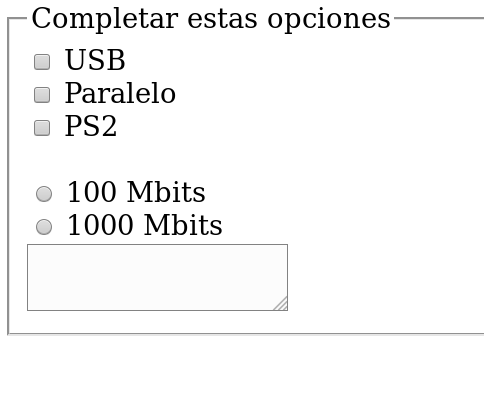
\includegraphics[scale=0.5]{examen-img/formulario.png}
\end{figure}
\begin{verbatim}
<form>
<fieldset>
  <legend>Completar estas opciones</legend>
  <input type='checkbox' name='conector' value='conectorusb'> USB   <br/>
  <input type='checkbox' name='conector' value='conectorparalelo'> Paralelo   <br/>
  <input type='checkbox' name='conector' value='conectorps2'> PS2   <br/>
  <br/>
  <input type='radio' name='velocidad' value='velocidad100_mbits'> 100 Mbits   <br/>
  <input type='radio' name='velocidad' value='velocidad1000_mbits'> 1000 Mbits   <br/>
<textarea id="informe"></textarea>
  <br/>
</fieldset>

</form>
\end{verbatim}
\end{document}
